\graphicspath{{../images/algorithm/}}
\chapter{Описание разработанного метода}

\section{Биологическое обоснование}
Как видно из предыдущей главы,  в настоящий момент при выборе аминокислот, подвергаемых точечному аланиновому мутагенезу, не проводится какой-либо сложный анализ.\todo{поправить}

% О-кольца
% фрагменты петель
% гидрофобность
% карманы

%\newpage
\subsection{Гидрофобность}
Широко известна и подтверждена гипотеза о том, что фолдинг белков происходит под влиянием свойств аминокислот: гидрофобные аминокислоты стремятся оказаться внутри, поскольку стараются избегать воду, которая находится снаружи от сворачивающейся молекулы \cite{hydrophoby}.

Похожим образом интерфейс взаимодействия цепочек, связь между ними образуется за счет гидрофобных взаимодействий: в область связывания попадают в первую очередь гидрофобные аминокислоты, находящиеся на поверхности цепочки белка.

%\newpage
\subsection{Карманы}
A complemented pocket is a concave surface
region on one protein chain that is filled by its
binding partner, representing a tight fit.
\cite{pockets2004}
%\newpage
\subsection{Петли}

Статья про петли\cite{loops2014}. Что там происходит: взята ASEdb, рассмотрены короткие фрагменты петель, содержащие энергетически горячие аминокислоты и приведена их какая-то классификация.
\subsection{Поиск по гомологии}
%\newpage
\section{Входные данные}

На входе PDB~\cite{pdb}, в каком виде данные. единицы измерения, точность
(полстраницы, возможно, с картинкой)
%\vspace{10cm}

\resizebox{0.8\textwidth}{!}{
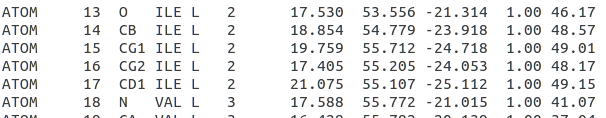
\includegraphics{atom_in_pdb.png}
}

PDB файл содержит информацию о белке, сгруппированную по следующим признакам: 
1. пространственное положение атомов аминокислот (секция ATOM):
включает информацию о координатах каждого из атомов, образующих аминокислоты, в свою очередь образующих цепочки белка или белков, вид атома, другие важные характеристики. Координаты упорядочены по положению аминокислот в цепочке.

2. информацию о вторичной структуре цепочек (секции helix, sheet)



%\newpage
\section{Выбор протяженных регионов}
Для того, чтобы выбрать протяженные регионы для аланинового сканирования, построим итеративный алгоритм.

Включим в состав множества протяженных регионов, содержащих ,,энергетически горячие аминокислотные остатки'', следующее:
\begin{itemize}
\item аминокислоты, образующие ,,интерфейс'' взаимодействия с парной цепочкой или белком (с использованием отсечки по расстоянию от второй цепочки)
\item аминокислоты, образующие поверхность ,,карманов'', находящихся в области взаимодействия пары белков
\item не-гидрофобные аминокислоты, являющиеся соседними по отношению к аминокислотам, образующим интерфейс
\item если интерфейс взаимодействия образован петлями, то добавим все аминокислоты, образующие петли 
\end{itemize}


%\newpage
\subsection{Формализация задачи}
\begin{frame}{Formal definitions - I}
\begin{itemize}
\item Protein molecule - a set of spheres S. Each sphere $s \in S,\,s=s(c_s, r_s)$ has center point $c_s$ and radius $r_s$, ,,atom'' corresponds to sphere.
\item the Euclidean distance $D(x,\,s)$ 
of a point $x$ from the surface of a sphere $s$:
$$
D(x,\,s) = || x - c_s || - r_s
$$

\item The minimal distance from the point x to the nearest
sphere (atom) is given by the function r (x):
$$
r(x) = \min \{D(x,s) | s \in S \}
$$
\end{itemize}
\end{frame}

\subsection{Маскировка аминокислот}

Исходя
\subsection{Триангуляция Делоне}
%\newpage
\subsection{Построение графа}
\begin{itemize}
\item Рассматриваем одновременно 2 цепочки, образующие белковый комплекс.
\item Начнем с построения выпуклой оболочки и триангуляции Делоне для каждой из них, будем искать протяженные регионы с энергетически горячими аминокислотными остатками  на одной из них. Строить будем по центрам атомов, формирующих аминокислоты цепочки.
\item Выберем все треугольники выпуклой оболочки, в которых хотя бы одна вершина удалена от некоторых атомов второй цепочки не далее, чем на выбранное (фиксированное) значение отсечки.
\end{itemize}


\begin{itemize}
\item Берется структура в PDB.
\item Центры атомов рассматриваются как точки. По ним строится триангуляция Делоне (с помощью scipy.delaunay - обертки над алгоритмом qhull).
\item Берется невзвешенная триангуляция -- по тем же соображениям, по которым она используется в CAVER (эвристика).
\end{itemize}
Я сопоставляю графу триангуляцию по тому же принципу, как в статье по CAVER:

\begin{center}
\resizebox{!}{0.3\textheight}{
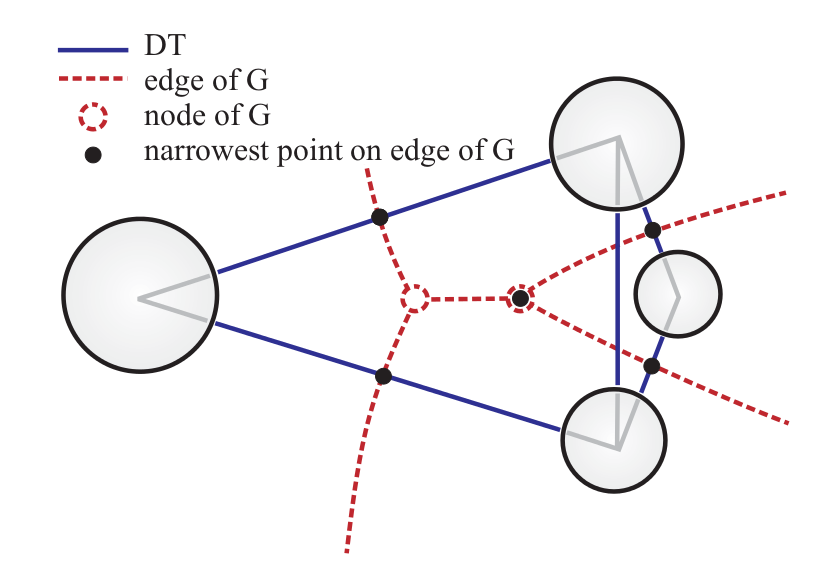
\includegraphics{image4_caver.png}
}

[Computation of tunnels in protein molecules using
Delaunay triangulation, P.Medek, et al., 2007]
\end{center}

Треугольники триангуляции -- вершины графа, ребра графа -- общие стороны треугольников (с ограничением снизу на длину).

Дополнительно используется такой же граф по треугольникам выпуклой оболочки (без ограничения снизу на длину стороны, просто по смежным по стороне треугольникам).

Выбирается начальное множество треугольников выпуклой оболочки. Сейчас берутся треугольники, вершины которых недалеко (в смысле отсечки по расстоянию) от второго белка.

%\newpage
\subsection{Псевдо-интерфейс}
\begin{itemize}
\item определяем множество треугольников выпуклой оболочки, для которых хотя бы одна вершина удалена от центров атомов второй цепочки не больше, чем на выбранное значение отсечки
\item Далее расширяем интерфейс
\begin{itemize}
\item шаг 1: добавляем к интерфейсу все треугольники выпуклой оболочки, содержащие атомы аминокислот, которые уже туда попали
\item шаг 2: продлеваем регион до границы гидрофобности
\item шаг 3: продлеваем регион за границы гидрофобности на 1 аминокислоту.
\end{itemize}
\end{itemize}


В результате у нас есть одна или нескольких протяженных связных областей выпуклой оболочки, по которым можно восстановить аминокислоты.
%\newpage
\subsection{Поиск карманов}
\todo{переписать}
Поиск карманов, каналов и полостей в макромолекулах является хорошо изученной задачей \cite{alpha_shapes1995, alpha_shapes1998, caver, ppi_kim2006}.  

\begin{itemize}
\item Начинаем с множества отобранных треугольников выпуклой оболочки (черным цветом)
\item Ищем в ширину с ограничениями
\item Ходим только по тем треугольникам, для которых ближайший треугольник выпуклой оболочки -- один из отобранных треугольников выпуклой оболочки, а не какой-либо из других треугольников выпуклой оболочки.
\item Ближайший треугольник == в смысле расстояния до ближайшей из вершин он ближе, чем другие треугольники выпуклой оболочки
\end{itemize}
\cite{alpha_shapes1995, alpha_shapes1998}
%\newpage
\subsection{Расширение интерфейса. Добавление петель}

Перед добавлением петель треугольники триангуляции преобразуются в фрагменты последовательности аминокислот, продлеваем их, используя информацию о вторичной структуре.


\begin{itemize}
\item Сейчас вторичная структура определяются на основе вывода DSSP \footnote{используется обертка к DSSP в составе biopython}.

Берутся непрерывные фрагменты структуры, которые не определяются как $\alpha$-спирали или $\beta$-листы, выбираю среди них те, в которые попадает какая-либо аминокислота, добавляются к выделяемому контуру.

%\todo{\item Я беру непрерывные фрагменты структуры, которые не определяются как альфа-спирали или бета-листы, выбираю среди них те, в которые попадает какая-либо аминокислота, ну и добавляю их к выделяемому контуру - технической сложности никакой.}

\end{itemize}


\begin{itemize}


%\todo{\item вариантов 2: либо не добавлять петли целиком, вместо этого добавлять только такие фрагменты (в статье они приведены), либо как-то их отмечать на выделенных петлях + отмечать на удаленных петлях, которые в выделенный регион не попали.}

% \todo{\item про HMM думаю, напишу через пару дней.}

% \todo{\item вообще если получится, я разберусь как считать взвешенную триангуляцию Делоне и с помощью нее искать карманы.}


\end{itemize}
